% Provenance (never printed): see sources/outline_sources.md (Year 2: Goldschmidt's
% classification; the chondritic Earth; core, mantle and crust compositions; trace
% elements and normalised diagrams). Curves from figdata/bachelor-2/geochem.py; exercise
% and problem values in the Book 4 scratch calculator calc/ch03.py.
\chapter{Os elementos na Terra}\label{ch:b2:elements-in-the-earth}

Uma tonelada das rochas dos continentes contém cerca de um miligrama e meio de
ouro. Uma tonelada dos \omterm{def:b2:planet-formation-meteorites:chondrule}{condritos carbonáceos} do capítulo anterior, as pedras mais
primitivas que caem do céu, contém cerca de cem vezes mais. A
Terra foi formada a partir de um material assim, portanto o ouro não falta à
Terra: ele está em outro lugar. Combinando as composições estimadas do núcleo e da
Terra silicática com a massa do núcleo, verifica-se que mais de 99 por cento do
ouro da Terra está no núcleo, para onde afundou com o ferro no início
da história da Terra. O ouro faz parte de uma família de elementos que acompanham o ferro
metálico; outros acompanham o sulfeto, outros a rocha silicática, e outros ainda escapam
para o ar. Este capítulo classifica os elementos nessas famílias, usa os
\omterm{def:b2:planet-formation-meteorites:chondrule}{condritos} para reconstituir a composição da Terra inteira e pesar seu
núcleo, descreve as composições do manto, da crosta oceânica e da
crosta continental, e apresenta os \omterm{def:b2:elements-in-the-earth:trace}{elementos-traço} e os diagramas nos quais
os geoquímicos leem a história de uma rocha.
% ledger: rg03:ucc-trace, lodders:ci-table, mcd03:core, ms95:pm-trace, data:prem

\begin{recall}
A Terra tem um núcleo metálico, principalmente de ferro, sob um manto silicático e uma fina
crosta; a sismologia dá o raio e a densidade de cada camada, e o núcleo
é de 5 a 10 por cento menos denso do que seria o ferro puro à mesma pressão e
temperatura, o que exige elementos leves nele: silício, enxofre, carbono,
oxigênio e hidrogênio são os candidatos (volume do primeiro ano). A
eletronegatividade de um elemento mede a força com que seus átomos atraem os
elétrons de uma ligação, e o raio de um íon depende de sua carga e do
número de seus vizinhos (química, no volume do primeiro ano). Um coeficiente de
partição é a razão entre as concentrações de uma substância em duas fases em
equilíbrio (química, no volume do primeiro ano). Os \omterm{def:b2:planet-formation-meteorites:chondrule}{condritos}, os \omterm{def:b2:planet-formation-meteorites:chondrule}{condritos
carbonáceos} e a \omterm{def:b2:planet-formation-meteorites:condensation}{sequência de condensação} foram apresentados no
\cref{ch:b2:planet-formation-meteorites}.
\end{recall}
% ledger: badro:core

\section{A classificação de Goldschmidt}

Quando um corpo condrítico funde, sua matéria se separa em líquidos imiscíveis: um
metal denso de ferro e níquel, um líquido sulfetado se houver enxofre suficiente, e um
fundido silicático, com uma fase gasosa acima. Cada elemento se distribui entre
essas fases segundo sua química, e a mesma partição é vista na
metalurgia, em que ferro fundido, um mate sulfetado e uma escória silicática se separam no
forno.

\begin{definition}[Classificação de Goldschmidt]
\label{def:b2:elements-in-the-earth:goldschmidt}
A \emph{classificação de Goldschmidt}\index{classificação de Goldschmidt} ordena
os elementos segundo a fase que eles preferem em um corpo que se separa em metal,
sulfeto, silicato e gás. Um \emph{elemento litófilo}\index{elemento litófilo}
prefere o silicato e o óxido; um \emph{elemento siderófilo}\index{elemento siderófilo}
prefere o ferro metálico; um \emph{elemento
calcófilo}\index{elemento calcófilo} prefere o sulfeto; um \emph{elemento
atmófilo}\index{elemento atmófilo} permanece no gás, como gás ou como composto
volátil.
\end{definition}

As classes seguem a química da ligação. Os \omterm{def:b2:elements-in-the-earth:goldschmidt}{elementos litófilos}, como os metais
alcalinos e alcalino-terrosos, o alumínio, o titânio ou as terras raras, cedem
facilmente seus elétrons ao oxigênio, que é muito mais eletronegativo, e
formam com ele ligações iônicas. Os \omterm{def:b2:elements-in-the-earth:goldschmidt}{elementos siderófilos}, os metais do grupo da platina, o ouro,
o níquel e o cobalto, têm eletronegatividades próximas da do ferro, ligam-se fracamente
ao oxigênio e se dissolvem no metal. Os \omterm{def:b2:elements-in-the-earth:goldschmidt}{elementos calcófilos}, entre eles o cobre, o zinco, o chumbo,
a prata e o cádmio, formam com o enxofre ligações mais covalentes.
Os \omterm{def:b2:elements-in-the-earth:goldschmidt}{elementos atmófilos} são os gases nobres, o nitrogênio e o hidrogênio. Muitos
elementos pertencem a duas classes, conforme as condições: o próprio ferro é
siderófilo em um corpo rico em metal e litófilo no manto oxidado, onde
fica na olivina e no piroxênio; o tungstênio e o molibdênio são siderófilos na
Terra, mas boa parte deles permaneceu no manto (figura abaixo).

\begin{omfigure}
\centering
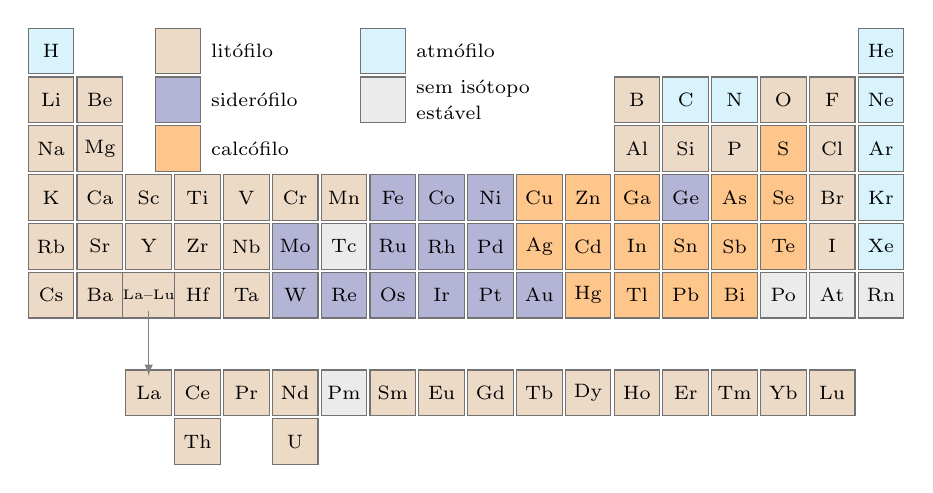
\begin{tikzpicture}[x=0.62cm, y=-0.62cm,
  lith/.style={fill=brown!30}, sid/.style={fill=blue!30!gray!45},
  chal/.style={fill=orange!45}, atm/.style={fill=cyan!15}, none/.style={fill=black!8},
  cell/.style={draw=black!55, minimum size=0.58cm, inner sep=0pt, font=\scriptsize}]
\foreach \s/\c/\r/\k in {H/1/1/atm, He/18/1/atm,
  Li/1/2/lith, Be/2/2/lith, B/13/2/lith, C/14/2/atm, N/15/2/atm, O/16/2/lith,
  F/17/2/lith, Ne/18/2/atm,
  Na/1/3/lith, Mg/2/3/lith, Al/13/3/lith, Si/14/3/lith, P/15/3/lith, S/16/3/chal,
  Cl/17/3/lith, Ar/18/3/atm,
  K/1/4/lith, Ca/2/4/lith, Sc/3/4/lith, Ti/4/4/lith, V/5/4/lith, Cr/6/4/lith,
  Mn/7/4/lith, Fe/8/4/sid, Co/9/4/sid, Ni/10/4/sid, Cu/11/4/chal, Zn/12/4/chal,
  Ga/13/4/chal, Ge/14/4/sid, As/15/4/chal, Se/16/4/chal, Br/17/4/lith, Kr/18/4/atm,
  Rb/1/5/lith, Sr/2/5/lith, Y/3/5/lith, Zr/4/5/lith, Nb/5/5/lith, Mo/6/5/sid,
  Tc/7/5/none, Ru/8/5/sid, Rh/9/5/sid, Pd/10/5/sid, Ag/11/5/chal, Cd/12/5/chal,
  In/13/5/chal, Sn/14/5/chal, Sb/15/5/chal, Te/16/5/chal, I/17/5/lith, Xe/18/5/atm,
  Cs/1/6/lith, Ba/2/6/lith, Hf/4/6/lith, Ta/5/6/lith, W/6/6/sid, Re/7/6/sid,
  Os/8/6/sid, Ir/9/6/sid, Pt/10/6/sid, Au/11/6/sid, Hg/12/6/chal, Tl/13/6/chal,
  Pb/14/6/chal, Bi/15/6/chal, Po/16/6/none, At/17/6/none, Rn/18/6/none,
  La/3/8/lith, Ce/4/8/lith, Pr/5/8/lith, Nd/6/8/lith, Pm/7/8/none, Sm/8/8/lith,
  Eu/9/8/lith, Gd/10/8/lith, Tb/11/8/lith, Dy/12/8/lith, Ho/13/8/lith,
  Er/14/8/lith, Tm/15/8/lith, Yb/16/8/lith, Lu/17/8/lith,
  Th/4/9/lith, U/6/9/lith}
  \node[cell, \k] at (\c,\r) {\s};
\node[cell, lith, minimum width=0.58cm] at (3,6) {\tiny La--Lu};
\draw[black!50, -latex] (3,6.32) -- (3,7.65);
% legend
\foreach \k/\t/\x/\y in {lith/litófilo/3.6/1, sid/siderófilo/3.6/2,
  chal/calcófilo/3.6/3, atm/atmófilo/7.8/1, none/{\shortstack[l]{sem isótopo\\estável}}/7.8/2}
  \node[cell, \k, label={[font=\scriptsize]east:\t}] at (\x,\y) {};
\end{tikzpicture}
\par\smallskip{\small As classes de Goldschmidt dos elementos estáveis e do tório e do urânio, cujos isótopos de vida longa sobrevivem desde o nascimento da Terra, coloridas segundo a classe
que domina na Terra; os elementos da fileira das terras raras ficam na caixa
La--Lu. Vários elementos pertencem a duas classes: o ferro, o níquel e o cobalto também são
litófilos no manto oxidado; o carbono também é siderófilo, e o fósforo,
siderófilo nos \omterm{def:b2:planet-formation-meteorites:fall-find}{meteoritos}.}
\end{omfigure}

\section{A Terra condrítica}

Ninguém pode amostrar a Terra como um todo: o núcleo está fora de alcance, e o
manto só chega à superfície em fragmentos. A composição da Terra total é
construída, em vez disso, a partir de dois conjuntos de indícios: os \omterm{def:b2:planet-formation-meteorites:fall-find}{meteoritos}, que amostram o
material a partir do qual os planetas se formaram, e as rochas do manto e os
fundidos que vêm dele.

\begin{definition}[Condrito CI]\label{def:b2:elements-in-the-earth:ci}
Um \emph{condrito CI}\index{condrito CI} é um membro do grupo de
\omterm{def:b2:planet-formation-meteorites:chondrule}{condritos carbonáceos} cujo nome vem do \omterm{def:b2:planet-formation-meteorites:fall-find}{meteorito} Ivuna: pedras negras e friáveis,
feitas quase inteiramente de matriz de grão fino, ricas em minerais hidratados e
em carbono, quase sem \omterm{def:b2:planet-formation-meteorites:chondrule}{côndrulos}. Exceto pelo hidrogênio, carbono, nitrogênio, oxigênio e os
gases nobres, sua composição é a mais próxima, entre todos os materiais conhecidos, da
fotosfera do Sol; eles são a composição de referência da geoquímica.
\end{definition}

O grupo conta cinco \omterm{def:b2:planet-formation-meteorites:fall-find}{meteoritos}, todos eles quedas: Alais (1806), Orgueil
(1864), Tonk (1911), Ivuna (1938) e Revelstoke (1965); Orgueil é o maior,
com catorze quilogramas. A composição adotada para o grupo é uma média ponderada
de suas análises, elemento por elemento; os valores usados neste capítulo são
citados onde são necessários.
% ledger: lodders:ci-table

\begin{definition}[Elementos refratários e voláteis]
\label{def:b2:elements-in-the-earth:volatility}
Um \emph{elemento refratário}\index{elemento refratário} é aquele cuja \omterm{def:b2:planet-formation-meteorites:condensation}{temperatura de condensação}
de 50 por cento (\cref{ch:b2:planet-formation-meteorites}) fica acima
das do magnésio, do silício e do ferro, \qtyrange{1310}{1340}{K} a
\qty{e-4}{bar}; um
\emph{elemento volátil}\index{elemento volátil} é aquele cuja \omterm{def:b2:planet-formation-meteorites:condensation}{temperatura de condensação}
fica abaixo delas.
\end{definition}

O teor de magnésio serve de padrão. O magnésio é litófilo, condensa-se
com a maior parte da rocha e não entra no núcleo, de modo que a razão entre um elemento
e o magnésio na Terra silicática, dividida pela mesma razão nos \omterm{def:b2:elements-in-the-earth:ci}{condritos CI},
mede quanto desse elemento a Terra silicática conservou em relação a um
material de partida condrítico. A água, o carbono e os outros compostos voláteis que
os \omterm{def:b2:elements-in-the-earth:ci}{condritos CI} contêm, e que a Terra não conservou, se cancelam na razão.

\begin{definition}[Terra silicática total, manto primitivo]
\label{def:b2:elements-in-the-earth:bse}
A \emph{Terra silicática total}\index{Terra silicática total} é a Terra sem
seu núcleo: manto, crosta, oceano e atmosfera tomados juntos, como seriam se
misturados. A mesma composição é chamada de \emph{manto primitivo}\index{manto primitivo}:
o manto tal como era depois da formação do núcleo e antes que qualquer crosta fosse
extraída dele.
\end{definition}

As estimativas do \omterm{def:b2:elements-in-the-earth:bse}{manto primitivo} baseiam-se nas rochas do manto que perderam
menos fundido, peridotitos trazidos como xenólitos em lavas (fotografia abaixo) ou
expostos em cadeias de montanhas, e na hipótese de que os \omterm{def:b2:elements-in-the-earth:goldschmidt}{elementos litófilos} refratários
estão em proporções condríticas entre si. Um resultado muito usado, com
magnésio 22.8, silício 21.0 e ferro 6.26 por cento em massa, é dado na
tabela de composições mais adiante.
% ledger: ms95:pm-trace, ms95:pm-oxides

\begin{omfigure}
\centering
\begin{minipage}{0.48\linewidth}
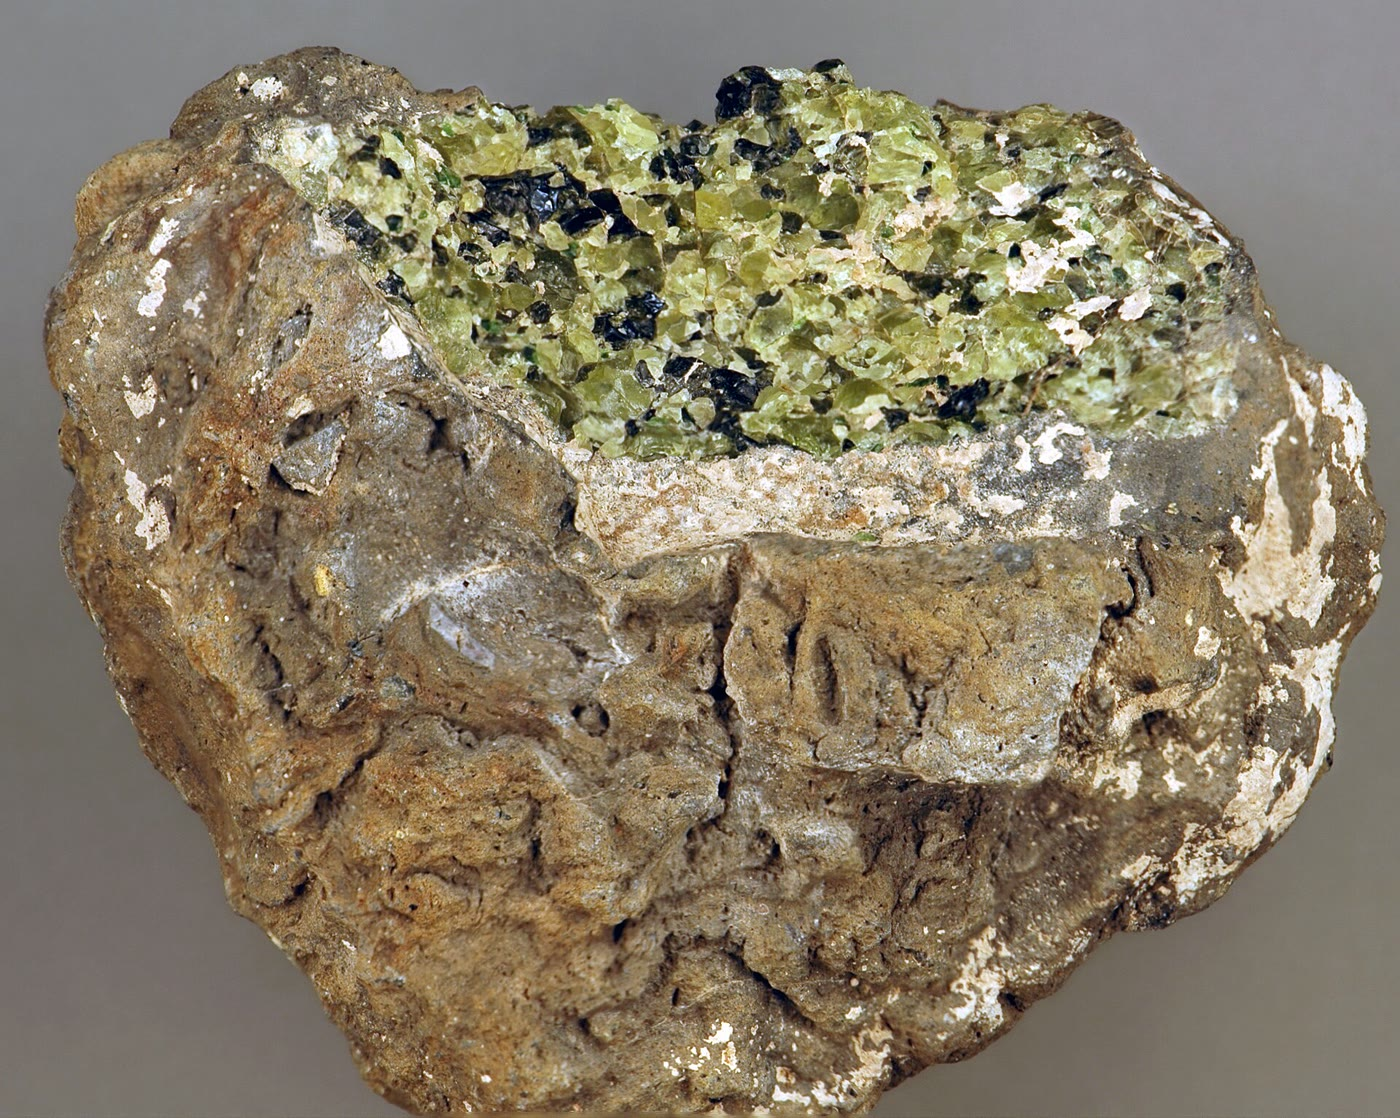
\includegraphics[width=\linewidth]{images/book4/b2-lherzolite-xenolith.jpg}
\end{minipage}\hfill
\begin{minipage}{0.48\linewidth}
{\small Um nódulo de peridotito do manto (lherzolito) em uma lava basáltica de
Kilbourne Hole, Novo México, com \qty{7.4}{cm} em sua maior largura: olivina
verde-amarelada com piroxênio escuro. A lava o arrancou do manto superior e o levou
até a superfície. James St.~John, CC BY 2.0.}
\end{minipage}
\end{omfigure}

A figura abaixo compara essa Terra silicática com os \omterm{def:b2:elements-in-the-earth:ci}{condritos CI}, elemento por
elemento, em função da \omterm{def:b2:planet-formation-meteorites:condensation}{temperatura de condensação} do capítulo anterior. Ela classifica
os elementos de um modo que nenhum outro indício permite. Os \omterm{def:b2:elements-in-the-earth:goldschmidt}{elementos litófilos}
refratários, do zircônio e das terras raras até o estrôncio e o bário, ficam todos
no mesmo nível, a menos de vinte por cento uns dos outros: a Terra silicática
conservou todos eles em suas proporções condríticas. Os \omterm{def:b2:elements-in-the-earth:goldschmidt}{elementos litófilos} voláteis
caem com sua \omterm{def:b2:planet-formation-meteorites:condensation}{temperatura de condensação}: cerca de um quinto do potássio
e do sódio, um décimo do rubídio, um centésimo do cloro e alguns
milésimos do bromo e do iodo estão presentes. Os \omterm{def:b2:elements-in-the-earth:goldschmidt}{elementos siderófilos} ficam muito abaixo de qualquer \omterm{def:b2:elements-in-the-earth:goldschmidt}{elemento litófilo}
de mesma volatilidade: a Terra silicática contém um sétimo de sua parte do
ferro, um treze avos do níquel e cerca de três milésimos dos
metais do grupo da platina e do ouro. Estes foram para o núcleo. Os \omterm{def:b2:elements-in-the-earth:goldschmidt}{elementos calcófilos},
em sua maioria também voláteis, são empobrecidos pelas duas razões.

\begin{omfigure}
\centering
\begin{tikzpicture}
\begin{axis}[omrecord, width=0.95\linewidth, height=8.2cm, ymode=log,
  xmin=500, xmax=1800, ymin=8e-4, ymax=3, x dir=reverse,
  xlabel={temperatura de condensação de 50 por cento a \qty{e-4}{bar} (K)},
  ylabel={$(X/\mathrm{Mg})_{\mathrm{BSE}}\,/\,(X/\mathrm{Mg})_{\mathrm{CI}}$},
  legend pos=south west, legend cell align=left, legend style={font=\scriptsize},
  tick label style={font=\scriptsize}, label style={font=\small},
  scaled x ticks=false, xticklabel style={/pgf/number format/1000 sep={}}]
\addplot[black!40, dashed, domain=500:1800, samples=2, forget plot] {1};
\addplot[only marks, mark=*, mark size=1.6pt, brown!70!black]
  table[x=T, y=ratio] {figdata/out/bachelor-2-geochem-volat-lith.dat};
\addlegendentry{litófilo}
\addplot[only marks, mark=square*, mark size=1.6pt, blue!60!black]
  table[x=T, y=ratio] {figdata/out/bachelor-2-geochem-volat-sid.dat};
\addlegendentry{siderófilo}
\addplot[only marks, mark=triangle*, mark size=2pt, orange!80!black]
  table[x=T, y=ratio] {figdata/out/bachelor-2-geochem-volat-chal.dat};
\addlegendentry{calcófilo}
\node[font=\tiny, brown!50!black, anchor=south] at (axis cs:1600,1.35)
  {Zr, Hf, Al, Sc, Y, Th, U, Ti, Ca, Sr, Ba, terras raras};
\begin{scope}[font=\tiny, brown!50!black]
\node[anchor=west] at (axis cs:1328,1.0) {Mg};
\node[anchor=north] at (axis cs:1310,0.80) {Si};
\node[anchor=west] at (axis cs:1150,0.23) {Mn};
\node[anchor=south] at (axis cs:1142,0.47) {Li};
\node[anchor=south] at (axis cs:1010,0.195) {K};
\node[anchor=north] at (axis cs:958,0.22) {Na};
\node[anchor=north] at (axis cs:908,0.175) {B};
\node[anchor=north] at (axis cs:800,0.116) {Rb};
\node[anchor=south] at (axis cs:734,0.175) {F};
\node[anchor=west] at (axis cs:795,0.0477) {Cs};
\node[anchor=west] at (axis cs:944,0.0102) {Cl};
\node[anchor=north] at (axis cs:546,0.0061) {Br};
\node[anchor=south] at (axis cs:535,0.0088) {I};
\end{scope}
\begin{scope}[font=\tiny, blue!50!black]
\node[anchor=west] at (axis cs:1325,0.144) {Fe};
\node[anchor=east] at (axis cs:1364,0.0775) {Ni};
\node[anchor=west] at (axis cs:1342,0.088) {Co};
\node[anchor=west] at (axis cs:1780,0.137) {W};
\node[anchor=south] at (axis cs:1590,0.0206) {Mo};
\node[anchor=north] at (axis cs:883,0.0139) {Ge};
\node[anchor=north] at (axis cs:1500,0.0026) {Re, Os, Ir, Ru, Pt, Pd};
\node[anchor=north] at (axis cs:1060,0.0026) {Au};
\end{scope}
\begin{scope}[font=\tiny, orange!60!black]
\node[anchor=west] at (axis cs:1030,0.0993) {Cu};
\node[anchor=north] at (axis cs:996,0.0167) {Ag};
\node[anchor=south] at (axis cs:726,0.0746) {Zn};
\node[anchor=south] at (axis cs:704,0.0325) {Sn};
\node[anchor=east] at (axis cs:735,0.0246) {Pb};
\node[anchor=west] at (axis cs:648,0.0249) {Cd};
\node[anchor=east] at (axis cs:715,0.0022) {Te};
\node[anchor=north] at (axis cs:690,0.0016) {Se};
\node[anchor=west] at (axis cs:660,0.0019) {S};
\end{scope}
\end{axis}
\end{tikzpicture}
\par\smallskip{\small A Terra silicática comparada com os \omterm{def:b2:elements-in-the-earth:ci}{condritos CI}: para cada elemento $X$, a
razão $X/\mathrm{Mg}$ na \omterm{def:b2:elements-in-the-earth:bse}{Terra silicática total} dividida pela mesma razão nos \omterm{def:b2:elements-in-the-earth:ci}{condritos
CI}, em função da \omterm{def:b2:planet-formation-meteorites:condensation}{temperatura de condensação} de 50 por cento (quente à esquerda).
Os \omterm{def:b2:elements-in-the-earth:goldschmidt}{elementos litófilos} refratários são condríticos entre si; os voláteis
são empobrecidos à medida que a \omterm{def:b2:planet-formation-meteorites:condensation}{temperatura de condensação} cai; os \omterm{def:b2:elements-in-the-earth:goldschmidt}{elementos siderófilos} e
calcófilos são muito mais empobrecidos. Dados: McDonough e Sun (1995);
Lodders (2003).}
\end{omfigure}
% ledger: ms95:pm-trace, lodders:ci-table, lodders:tc-table, lodders:tc-more

Os \omterm{def:b2:elements-in-the-earth:goldschmidt}{elementos litófilos} refratários ficam cerca de 15 por cento acima do magnésio. Os
dois não podem ser ambos exatamente condríticos: ou a Terra ganhou \omterm{def:b2:elements-in-the-earth:volatility}{elementos
refratários}, ou perdeu um pouco de magnésio, ou o magnésio do modelo está
subestimado (\cref{exo:b2:elements-in-the-earth:12}). O silício, com 0.83, fica ainda mais abaixo do
nível refratário; parte do silício que falta pode estar no núcleo (problema).

Os \omterm{def:b2:elements-in-the-earth:goldschmidt}{elementos siderófilos} da Terra silicática, combinados com uma Terra total
condrítica, pesam o núcleo. Suponha-se que a Terra total tenha a razão CI $r_X = X/\mathrm{Mg}$
para um \omterm{def:b2:elements-in-the-earth:goldschmidt}{elemento siderófilo} $X$, e que o núcleo contenha a concentração $c_X$ dele,
mas nenhum magnésio.

\begin{proposition}[Fração mássica do núcleo a partir de uma razão condrítica]
\label{prop:b2:elements-in-the-earth:core}
Sejam $x$ a fração mássica do núcleo, $C_X$ e $C_{\mathrm{Mg}}$ as
concentrações de $X$ e de magnésio na Terra silicática, e $c_X$ a de $X$ no
núcleo. Se a Terra tem a razão condrítica $r_X$, então
\[
  \frac{x}{1-x} = \frac{r_X C_{\mathrm{Mg}} - C_X}{c_X}.
\]
\end{proposition}

\begin{proof}
Uma massa $M$ de Terra contém $(1-x)MC_X + xMc_X$ de $X$ e $(1-x)MC_{\mathrm{Mg}}$ de
magnésio. Sua razão é $r_X$:
$(1-x)C_X + xc_X = r_X(1-x)C_{\mathrm{Mg}}$. Dividir por $(1-x)c_X$ dá o
resultado.
\end{proof}

Com o ferro, $r_{\mathrm{Fe}} = \num{182800}/\num{95870} = 1.907$ nos \omterm{def:b2:elements-in-the-earth:ci}{condritos CI},
22.8 por cento de magnésio e 6.26 por cento de ferro na Terra silicática, e 85.5 por
cento de ferro em um núcleo modelo, a proposição dá $x/(1-x) = 0.435$, um núcleo de 30
por cento da massa da Terra. A sismologia, integrando a densidade do
modelo de referência da Terra, dá 32.5 por cento. A concordância a menos de um décimo
apoia a imagem de uma Terra condrítica cujo ferro está principalmente no núcleo; a
diferença mede quanto a razão ferro/magnésio da Terra se afasta da
razão condrítica (problema). O mesmo balanço diz onde está cada elemento da Terra
(figura abaixo): quase toda a sua platina, seu irídio e seu ouro, e a maior parte de seu ferro,
seu níquel e seu enxofre, estão no núcleo.
% ledger: lodders:ci-table, ms95:pm-trace, mcd03:core, data:prem

\begin{omfigure}
\centering
\begin{tikzpicture}
\begin{axis}[omrecord, xbar, width=0.8\linewidth, height=6.4cm, bar width=5pt,
  xmin=0, xmax=100, ymin=0.4, ymax=14.6, y dir=reverse,
  ytick={1,...,14}, yticklabels from table={figdata/out/bachelor-2-geochem-budget.dat}{el},
  xlabel={parcela do inventário da Terra contida no núcleo (por cento)},
  tick label style={font=\scriptsize}, label style={font=\small},
  nodes near coords, nodes near coords align={horizontal},
  every node near coord/.append style={font=\tiny, /pgf/number format/fixed,
    /pgf/number format/precision=1}]
\addplot[fill=blue!35!gray!50, draw=black!60]
  table[x=share, y=idx] {figdata/out/bachelor-2-geochem-budget.dat};
\end{axis}
\end{tikzpicture}
\par\smallskip{\small Onde estão os elementos da Terra: a parcela de cada elemento contida no
núcleo, a partir de uma composição modelo do núcleo, do \omterm{def:b2:elements-in-the-earth:bse}{manto primitivo} e de um núcleo de 32.5
por cento da massa da Terra. Dados: McDonough (2003); McDonough e Sun (1995);
modelo de referência da Terra.}
\end{omfigure}
% ledger: mcd03:core, ms95:pm-trace, data:prem

\section{Manto e crostas}

A Terra silicática está dividida, desde sua formação, em um manto e dois
tipos de crosta. A crosta oceânica é produzida pela fusão do manto sob as
dorsais meso-oceânicas; a crosta continental, por uma longa história de fusão acima das
zonas de subducção, de retrabalhamento e de erosão (capítulos posteriores). Dois fundidos de referência
do manto ancoram a discussão.

\begin{definition}[Basalto de dorsal meso-oceânica, basalto de ilha oceânica]
\label{def:b2:elements-in-the-earth:morb-oib}
Um \emph{basalto de dorsal meso-oceânica}\index{basalto de dorsal meso-oceânica} (MORB) é um basalto
extravasado em uma dorsal meso-oceânica, a rocha do topo da crosta oceânica. Um
\emph{basalto de ilha oceânica}\index{basalto de ilha oceânica} (OIB) é um basalto extravasado
em um vulcão oceânico afastado dos limites de placas, como os do Havaí,
comumente atribuído a uma pluma do manto (volume do primeiro ano).
\end{definition}

O MORB médio da tabela abaixo é uma média global construída a partir de 771 segmentos
de dorsal, cada segmento ponderado por seu comprimento e sua taxa de expansão, de modo que a
média represente a crosta que as dorsais produzem. A coluna OIB
é uma única rocha: o material de referência basáltico BHVO-2, coletado em 1995
de uma lava que transbordou da cratera Halemaumau do Kilauea, no Havaí, em 1919,
e analisado por muitos laboratórios, de modo que a maior parte de suas terras raras é conhecida a
cerca de um por cento. A crosta continental superior é uma média estimada a partir de
rochas e sedimentos da superfície.
% ledger: gale13:allmorb, usgs:bhvo2-origin, usgs:bhvo2-major, rg14:crust

\begin{table}[h]
\centering
\small
\begin{tabular}{lrrrr}
\hline
óxido (\%\,em massa) & \omterm{def:b2:elements-in-the-earth:bse}{manto primitivo} & MORB & OIB (BHVO-2) & crosta cont.\ superior\\
\hline
\ce{SiO2} & 45.0 & 50.47 & 49.60 & 66.6\\
\ce{TiO2} & 0.201 & 1.68 & 2.731 & 0.64\\
\ce{Al2O3} & 4.45 & 14.70 & 13.44 & 15.4\\
FeO (total) & 8.05 & 10.43 & 11.15 & 5.04\\
MnO & 0.135 & 0.184 & 0.1690 & 0.10\\
MgO & 37.8 & 7.58 & 7.257 & 2.48\\
CaO & 3.55 & 11.39 & 11.40 & 3.59\\
\ce{Na2O} & 0.36 & 2.79 & 2.219 & 3.27\\
\ce{K2O} & 0.029 & 0.160 & 0.5130 & 2.80\\
\ce{P2O5} & 0.021 & 0.184 & 0.2685 & 0.15\\
\hline
\end{tabular}
\caption{Composições em elementos maiores de quatro reservatórios. O BHVO-2 dá seu ferro como
\ce{Fe2O3} (12.39 por cento), aqui convertido em FeO. Dados: McDonough e Sun
(1995); Gale e colaboradores (2013); ficha informativa do USGS para o BHVO-2; Rudnick e
Gao (2014).}
\label{tab:b2:elements-in-the-earth:majors}
\end{table}
% ledger: ms95:pm-oxides, gale13:allmorb, usgs:bhvo2-major, rg14:crust

Lida da esquerda para a direita, a tabela conta a história da fusão. O manto é um peridotito
rico em magnésio, com quase 38 por cento de MgO e menos de 5 por cento de \ce{Al2O3} e de CaO.
Seus fundidos, os basaltos, contêm cinco vezes menos magnésio e três vezes mais
cálcio e alumínio: os elementos que entram facilmente no fundido deixam o manto
primeiro. O potássio, o sódio e o titânio são ainda mais ricos nos fundidos em comparação
com o manto, e o potássio é o mais rico de todos na crosta continental,
com quase cem vezes sua concentração no \omterm{def:b2:elements-in-the-earth:bse}{manto primitivo}. O silício sobe
do manto para os basaltos só um pouco, e muito mais na crosta
continental, cuja média é próxima da de um granodiorito.

\section{Elementos-traço}

Dez óxidos perfazem cerca de 99 por cento de cada rocha da tabela acima. Os demais elementos,
presentes em partes por milhão, seguem os mesmos processos que os maiores, mas
são muito mais sensíveis a eles.

\begin{definition}[Elemento-traço]\label{def:b2:elements-in-the-earth:trace}
Um \emph{elemento-traço}\index{elemento-traço} de uma rocha é um elemento cuja
concentração fica, por convenção, abaixo de 0.1 por cento em massa (\qty{1000}{ppm}).
Os elementos-traço raramente formam minerais próprios; eles substituem elementos
maiores nos sítios das redes cristalinas.
\end{definition}

Um \omterm{def:b2:elements-in-the-earth:trace}{elemento-traço} é tão diluído que sua própria concentração não altera os
cristais nem o fundido: sua distribuição entre eles é então uma simples razão,
independente de sua concentração em uma ampla faixa.

\begin{definition}[Coeficiente de partição mineral--fundido; elementos compatíveis e
incompatíveis]\label{def:b2:elements-in-the-earth:partition}
O \emph{coeficiente de partição mineral--fundido}\index{coeficiente de partição mineral--fundido}
de um elemento em um mineral é a razão entre suas concentrações no
mineral e em um fundido silicático em equilíbrio com ele,
$D = C_{\mathrm{mineral}}/C_{\mathrm{melt}}$. Para uma rocha de vários minerais de
frações mássicas $x_i$, o \emph{coeficiente de partição global} é
$\bar D = C_{\mathrm{rock}}/C_{\mathrm{melt}}$. Um elemento é um
\emph{elemento compatível}\index{elemento compatível} em uma rocha se $\bar D > 1$,
e um \emph{elemento incompatível}\index{elemento incompatível} se $\bar D < 1$.
\end{definition}

\begin{proposition}[Coeficiente de partição global]
\label{prop:b2:elements-in-the-earth:bulk-d}
Se cada mineral da rocha está em equilíbrio com o mesmo fundido, o coeficiente
de partição global é a média dos coeficientes dos minerais ponderada pelas
frações mássicas: $\bar D = \sum_i x_i D_i$.
\end{proposition}

\begin{proof}
A rocha contém $C_{\mathrm{rock}} = \sum_i x_i C_i$, e cada mineral
$C_i = D_i C_{\mathrm{melt}}$. Dividir por $C_{\mathrm{melt}}$ dá o resultado.
\end{proof}

Se um íon cabe em um sítio depende de seu raio e de sua carga. Um íon próximo em
raio e carga do íon maior de um sítio, como o \ce{Ni^2+} no lugar do \ce{Mg^2+} na
olivina, entra facilmente e é compatível. Um íon muito maior, como o
\ce{Rb+} ou o \ce{Ba^2+}, ou mais carregado, como o \ce{Zr^4+} ou o
\ce{Nb^5+}, deforma a rede e é rejeitado para o fundido: ele é
incompatível nos minerais do manto. Dois grupos de \omterm{def:b2:elements-in-the-earth:partition}{elementos incompatíveis}
comportam-se de modo diferente mais adiante, quando a água intervém.

\begin{definition}[Elementos litófilos de grande raio iônico e elementos de alta intensidade de campo]
\label{def:b2:elements-in-the-earth:lile-hfse}
Os \emph{elementos litófilos de grande raio iônico}\index{elemento litófilo de grande raio iônico}
(LILE) são \omterm{def:b2:elements-in-the-earth:partition}{elementos incompatíveis} de íons grandes e de carga baixa, $+1$ ou $+2$:
potássio, rubídio, césio, estrôncio, bário. Os
\emph{elementos de alta intensidade de campo}\index{elemento de alta intensidade de campo} (HFSE)
são \omterm{def:b2:elements-in-the-earth:partition}{elementos incompatíveis} de íons pequenos e muito carregados, $+4$ ou $+5$:
zircônio, háfnio, nióbio, tântalo, titânio.
\end{definition}

Os LILE se dissolvem facilmente em fluidos ricos em água; os HFSE, quase nada. Uma rocha
alterada pela água, ou um fundido que herdou fluidos, como acima das zonas de subducção,
leva portanto LILE com pouco HFSE.

\begin{definition}[Elementos terras raras]\label{def:b2:elements-in-the-earth:ree}
Os \emph{elementos terras raras}\index{elemento terra rara} (ETR) são os quinze
lantanídeos, do lantânio ao lutécio; o promécio não tem isótopo estável. Todos
são litófilos e refratários, quase todos trivalentes, e seu raio iônico
diminui regularmente do lantânio ao lutécio; o európio também pode ser divalente em
fundidos reduzidos.
\end{definition}

Como as terras raras diferem gradualmente em raio e em nada mais, elas
se fracionam gradualmente: as leves, do lantânio ao samário, são as menos
compatíveis; as pesadas, do gadolínio ao lutécio, cabem melhor em alguns
minerais, sobretudo na granada (figura abaixo). Em uma rocha com granada, as terras raras
pesadas tornam-se compatíveis: um fundido dessa rocha é rico em terras raras leves e
pobre em pesadas.

\begin{omfigure}
\centering
\begin{tikzpicture}
\begin{axis}[omrecord, width=0.78\linewidth, height=6.4cm, ymode=log,
  xmin=0.6, xmax=9.4, ymin=5e-4, ymax=20,
  xtick={1,...,9}, xticklabels from table={figdata/out/bachelor-2-geochem-dvals.dat}{el},
  ylabel={coeficiente de partição $D$}, legend pos=south east,
  legend cell align=left, legend style={font=\scriptsize},
  tick label style={font=\scriptsize}, label style={font=\small}]
\addplot[black!40, dashed, domain=0.6:9.4, samples=2, forget plot] {1};
\addplot[thick, green!45!black, mark=*] table[x=idx, y=cpx] {figdata/out/bachelor-2-geochem-dvals.dat};
\addlegendentry{clinopiroxênio}
\addplot[thick, red!70!black, mark=square*] table[x=idx, y=gar] {figdata/out/bachelor-2-geochem-dvals.dat};
\addlegendentry{granada}
\addplot[thick, olive!70!black, mark=triangle*] table[x=idx, y=ol] {figdata/out/bachelor-2-geochem-dvals.dat};
\addlegendentry{olivina + ortopiroxênio + espinélio}
\addplot[very thick, black, mark=diamond*] table[x=idx, y=bulk] {figdata/out/bachelor-2-geochem-dvals.dat};
\addlegendentry{rocha total (65/18/17 por cento)}
\node[font=\scriptsize, anchor=south west] at (axis cs:0.7,1) {compatível};
\node[font=\scriptsize, anchor=north west] at (axis cs:0.7,1) {incompatível};
\end{axis}
\end{tikzpicture}
\par\smallskip{\small \omterm{def:b2:elements-in-the-earth:partition}{Coeficientes de partição mineral--fundido} das terras raras para o
clinopiroxênio, a granada e uma mistura de olivina, ortopiroxênio e espinélio, e o
coeficiente global de um granada-piroxenito com 65 por cento de clinopiroxênio, 18 por
cento de granada e 17 por cento dos outros minerais (proposição acima). A granada
torna compatíveis as terras raras pesadas. Dados: Budahn (1991).}
\end{omfigure}
% ledger: budahn91:d-ree, budahn91:modes

\section{Diagramas normalizados}

As abundâncias de elementos vizinhos diferem por fatores grandes por causa da
história nuclear da matéria: os elementos de número atômico par são mais abundantes que
seus vizinhos ímpares, como mostra a coluna CI das terras raras (lantânio 0.232,
cério 0.621, praseodímio 0.0928 ppm). Plotadas em valores brutos, as terras raras de uma rocha formam um
dente de serra que esconde sua história geológica. Dividir por uma referência o elimina.
% ledger: lodders:ci-table

\begin{definition}[Diagrama normalizado]\label{def:b2:elements-in-the-earth:normalised}
Um \emph{diagrama normalizado}\index{diagrama normalizado} representa, para uma série de
elementos em uma ordem fixa, a concentração em uma amostra dividida pela concentração em uma
referência, $X_N = C_X/C_X^{\mathrm{ref}}$, em escala logarítmica. As terras raras
são normalizadas aos \omterm{def:b2:elements-in-the-earth:ci}{condritos CI} na ordem do número atômico; um conjunto mais longo de
\omterm{def:b2:elements-in-the-earth:partition}{elementos incompatíveis}, muitas vezes chamado de diagrama aranha, é normalizado ao
\omterm{def:b2:elements-in-the-earth:bse}{manto primitivo} e ordenado por incompatibilidade decrescente na fusão do manto.
\end{definition}

Uma amostra com as mesmas proporções que a referência aparece como uma linha horizontal;
sua altura dá o enriquecimento. Uma inclinação mostra um fracionamento entre elementos leves e
pesados, medido por uma razão como $(\mathrm{La}/\mathrm{Yb})_N$. Um
único elemento fora da linha é uma anomalia.

\begin{proposition}[Anomalia de európio]\label{prop:b2:elements-in-the-earth:normalised}
Em um \omterm{def:b2:elements-in-the-earth:normalised}{diagrama normalizado} em que o padrão é uma reta em
$\log X_N$ entre o samário e o gadolínio, o valor esperado para o európio, que
fica no meio, é $\mathrm{Eu}^* = \sqrt{\mathrm{Sm}_N\,\mathrm{Gd}_N}$. A
\emph{anomalia de európio}\index{anomalia de európio} é
$\mathrm{Eu}/\mathrm{Eu}^* = \mathrm{Eu}_N/\sqrt{\mathrm{Sm}_N\,\mathrm{Gd}_N}$:
abaixo de 1 ela é negativa, acima de 1, positiva.
\end{proposition}

\begin{proof}
Samário, európio e gadolínio são consecutivos, a passos iguais ao longo do eixo.
Uma reta em $\log X_N$ assume no ponto do meio a média dos valores das extremidades:
$\log \mathrm{Eu}^* = \tfrac12(\log \mathrm{Sm}_N + \log \mathrm{Gd}_N)$, o
logaritmo da média geométrica.
\end{proof}

O európio é a única terra rara que pode ser divalente. O \ce{Eu^2+} tem quase o
raio do \ce{Ca^2+} e do \ce{Sr^2+}, de modo que o feldspato plagioclásio o aceita onde
rejeita as terras raras trivalentes. Um fundido do qual o plagioclásio cristalizou
tem uma anomalia negativa; a rocha rica em plagioclásio deixada para trás, uma positiva.

\begin{omfigure}
\centering
\begin{tikzpicture}
\begin{axis}[omrecord, width=0.8\linewidth, height=6.4cm, ymode=log,
  xmin=0.6, xmax=13.4, ymin=5, ymax=250,
  xtick={1,...,13}, xticklabels from table={figdata/out/bachelor-2-geochem-ree.dat}{el},
  ylabel={amostra / condrito CI}, legend pos=north east, legend cell align=left,
  legend style={font=\scriptsize}, tick label style={font=\scriptsize},
  label style={font=\small}]
\addplot[thick, blue!70!black, mark=*] table[x=idx, y=morb] {figdata/out/bachelor-2-geochem-ree.dat};
\addlegendentry{MORB médio}
\addplot[thick, red!70!black, mark=square*] table[x=idx, y=oib] {figdata/out/bachelor-2-geochem-ree.dat};
\addlegendentry{OIB (BHVO-2, Havaí)}
\addplot[thick, brown!70!black, mark=triangle*] table[x=idx, y=ucc] {figdata/out/bachelor-2-geochem-ree.dat};
\addlegendentry{crosta continental superior}
\end{axis}
\end{tikzpicture}
\par\smallskip{\small Padrões de terras raras normalizados aos \omterm{def:b2:elements-in-the-earth:ci}{condritos CI} (túlio omitido, por
falta de um valor do MORB). O MORB médio é plano, ligeiramente mais pobre nas terras raras
leves; o basalto havaiano é enriquecido nelas; a crosta superior é fortemente
enriquecida nelas, com uma anomalia negativa de európio. Dados: Gale e colaboradores
(2013); ficha BHVO-2 do USGS; Rudnick e Gao; Lodders (2003).}
\end{omfigure}
% ledger: gale13:allmorb, usgs:bhvo2-trace, rg03:ucc-trace, lodders:ci-table

Os três padrões da figura acima se leem como três histórias. O MORB médio
fica cerca de 25 vezes acima do \omterm{def:b2:planet-formation-meteorites:chondrule}{condrito}, quase plano, com $(\mathrm{La}/\mathrm{Sm})_N
= 0.85$: sua fonte mantélica já havia perdido parte de seus elementos mais incompatíveis
para fundidos anteriores, entre eles a crosta continental. O basalto havaiano é
enriquecido nas terras raras leves, $(\mathrm{La}/\mathrm{Yb})_N = 5.4$, e suas
terras raras pesadas são mais baixas que as do MORB: ele veio de um grau menor de
fusão, no qual a granada ficou para trás retendo as pesadas. A crosta
continental superior é enriquecida mais de cem vezes em lantânio, com
$(\mathrm{La}/\mathrm{Yb})_N = 10.9$ e $\mathrm{Eu}/\mathrm{Eu}^* = 0.72$: ela é
o produto de fusões repetidas, e seu déficit de európio é compatível com
plagioclásio deixado para trás na crosta profunda.

\begin{omfigure}
\centering
\begin{tikzpicture}
\begin{axis}[omrecord, width=\linewidth, height=6.6cm, ymode=log,
  xmin=0.5, xmax=27.5, ymin=1, ymax=400,
  xtick={1,...,27}, xticklabels from table={figdata/out/bachelor-2-geochem-spider.dat}{el},
  ylabel={amostra / manto primitivo}, legend pos=north east, legend cell align=left,
  legend style={font=\scriptsize}, tick label style={font=\scriptsize},
  label style={font=\small}]
\addplot[thick, blue!70!black, mark=*, mark size=1.4pt] table[x=idx, y=morb] {figdata/out/bachelor-2-geochem-spider.dat};
\addlegendentry{MORB médio}
\addplot[thick, red!70!black, mark=square*, mark size=1.4pt] table[x=idx, y=oib] {figdata/out/bachelor-2-geochem-spider.dat};
\addlegendentry{OIB (BHVO-2)}
\addplot[thick, brown!70!black, mark=triangle*, mark size=1.6pt] table[x=idx, y=ucc] {figdata/out/bachelor-2-geochem-spider.dat};
\addlegendentry{crosta continental superior}
\end{axis}
\end{tikzpicture}
\par\smallskip{\small \omterm{def:b2:elements-in-the-earth:partition}{Elementos incompatíveis} normalizados ao \omterm{def:b2:elements-in-the-earth:bse}{manto primitivo}, do mais
incompatível à esquerda. A crosta continental mostra os LILE altos, os vales
profundos no nióbio, no tântalo e no titânio e o pico de chumbo herdados da
fusão nas zonas de subducção; o basalto havaiano mostra uma corcova no nióbio e no
tântalo. Potássio e titânio calculados a partir dos óxidos. Dados: como na figura das terras
raras; McDonough e Sun (1995).}
\end{omfigure}
% ledger: gale13:allmorb, usgs:bhvo2-trace, usgs:bhvo2-major, rg03:ucc-trace, ms95:pm-trace

O diagrama aranha acima acentua o contraste. Na crosta continental,
o nióbio e o tântalo ficam muito abaixo de seus vizinhos tório e lantânio,
o titânio abaixo de seus vizinhos, e o chumbo bem acima: $(\mathrm{Nb}/\mathrm{La})_N =
0.38$. No basalto havaiano, a mesma razão é 1.17, e no MORB médio,
0.99. O padrão da crosta é a assinatura dos fundidos acima das zonas de subducção, onde
fluidos levaram os LILE e o chumbo para a cunha mantélica e deixaram os HFSE para trás
(capítulos posteriores); os \omterm{def:b2:elements-in-the-earth:morb-oib}{basaltos de ilha oceânica} não a têm. O diagrama aranha de uma única amostra
pode, portanto, distinguir uma lava de arco de uma lava de ilha oceânica, ou revelar um basalto
contaminado por crosta continental (\cref{exo:b2:elements-in-the-earth:11}).

\begin{inthelab}[De uma rocha a uma lista de elementos-traço]
\begin{minipage}[t]{0.6\linewidth}
\vspace{0pt}
Um geoquímico que quer os \omterm{def:b2:elements-in-the-earth:trace}{elementos-traço} de um basalto parte de algumas centenas de
gramas de seu interior mais fresco, livre de crosta de alteração e de veios. A rocha é
britada e depois moída até um pó fino em um moinho cujo material não
contamina os elementos de interesse. Uma pequena porção do pó é posta
em solução com ácidos, ou fundida com um fundente, e a solução é analisada por
espectrometria de massa com plasma indutivamente acoplado, que mede a maior parte dos
elementos do diagrama aranha de uma só vez. A cada lote de amostras, o
laboratório analisa materiais de referência de composição conhecida, como o
basalto havaiano BHVO-2: seus valores vêm de um estudo que combinou as médias de
muitos laboratórios, 132 deles para o lantânio, e alguns deles, como os
valores de neodímio e samário, por diluição isotópica, que conta os átomos de
um elemento em relação a uma quantidade conhecida, adicionada, de um de seus isótopos. Se o resultado do laboratório para o material de referência ficar
dentro da incerteza do valor aceito, os resultados das amostras desconhecidas
são aceitos com ele.
\end{minipage}\hfill
\begin{minipage}[t]{0.36\linewidth}
\vspace{0pt}
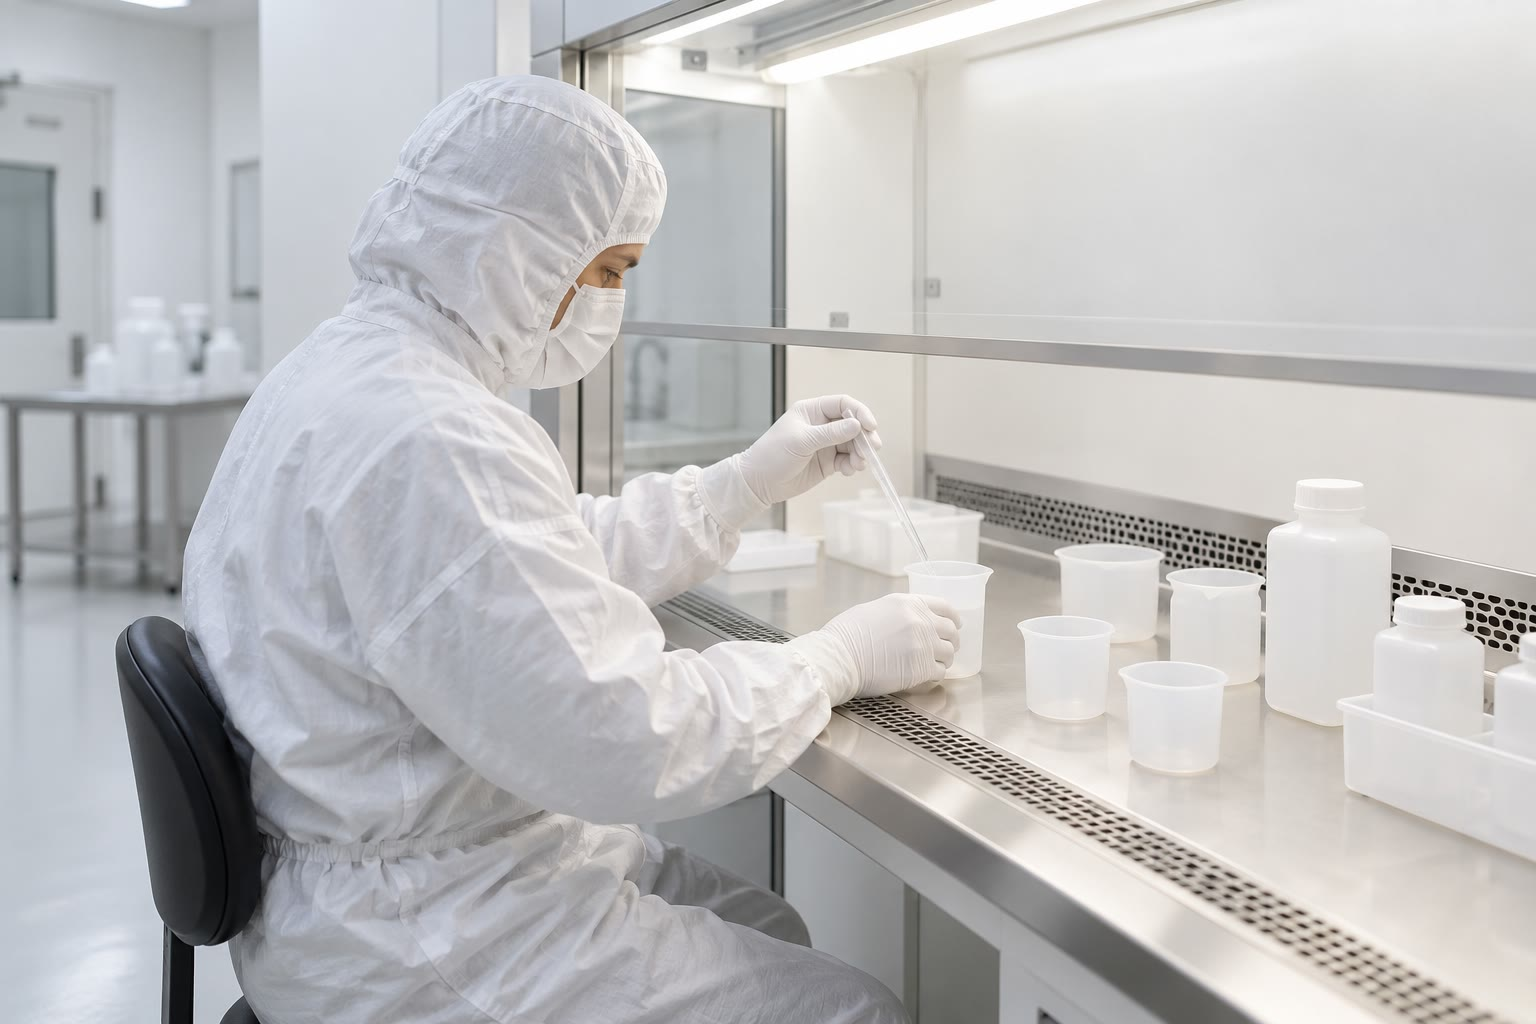
\includegraphics[width=\linewidth]{images/book4/ai/b2-clean-lab.jpg}

\smallskip
{\footnotesize Um trabalhador com traje de sala limpa na bancada de fluxo laminar de um
laboratório limpo de geoquímica (ilustração gerada por IA).\par}
\end{minipage}
\end{inthelab}
% ledger: usgs:bhvo2-trace, usgs:bhvo2-origin

\section{Exercícios}

\begin{exercise}[$\star$]\label{exo:b2:elements-in-the-earth:1}
O basalto BHVO-2 contém 0.5130 por cento de \ce{K2O} e 2.731 por cento de \ce{TiO2}
em massa. Com as massas atômicas K 39.10, Ti 47.87 e O 16.00, calcule seus
teores de potássio e de titânio em ppm.
\end{exercise}

\begin{exercise}[$\star$]\label{exo:b2:elements-in-the-earth:2}
Na \omterm{def:b2:elements-in-the-earth:bse}{Terra silicática total}, as razões $(X/\mathrm{Mg})$ divididas pelas razões CI
valem 1.16 para o alumínio, 0.22 para o sódio, 0.077 para o níquel e 0.0029 para o
irídio. As \omterm{def:b2:planet-formation-meteorites:condensation}{temperaturas de condensação} desses elementos são 1653, 958, 1353
e \qty{1603}{K}. Dê a classe de Goldschmidt de cada elemento e explique cada
empobrecimento.
\end{exercise}

\begin{exercise}[$\star$]\label{exo:b2:elements-in-the-earth:3}
A crosta continental superior contém \qty{31}{ppm} de lantânio e \qty{2.0}{ppm}
de itérbio; os \omterm{def:b2:elements-in-the-earth:ci}{condritos CI}, 0.232 e \qty{0.163}{ppm}. Calcule os
valores normalizados ao \omterm{def:b2:planet-formation-meteorites:chondrule}{condrito} e $(\mathrm{La}/\mathrm{Yb})_N$. O que a
razão diz sobre a crosta?
\end{exercise}

\begin{exercise}[$\star$]\label{exo:b2:elements-in-the-earth:4}
A crosta continental superior contém 4.7, 1.0 e \qty{4.0}{ppm} de samário,
európio e gadolínio; os \omterm{def:b2:elements-in-the-earth:ci}{condritos CI}, 0.145, 0.0546 e \qty{0.198}{ppm}.
Calcule $\mathrm{Eu}/\mathrm{Eu}^*$. Que mineral explica o resultado?
\end{exercise}

\begin{exercise}[$\star\star$]\label{exo:b2:elements-in-the-earth:5}
Um granada-piroxenito é feito de 65 por cento de clinopiroxênio, 18 por cento de granada e
17 por cento de olivina, ortopiroxênio e espinélio. Os coeficientes de partição do
lantânio são 0.058, 0.001 e 0.001; os do lutécio, 0.53, 5.8 e 0.18.
Calcule os coeficientes globais. Que elemento é compatível na rocha? Que
mineral contém a maior parte do lutécio da rocha?
\end{exercise}

\begin{exercise}[$\star\star$]\label{exo:b2:elements-in-the-earth:6}
A \omterm{def:b2:elements-in-the-earth:bse}{Terra silicática total} contém 22.8 por cento de magnésio, \qty{2670}{ppm} de
sódio e \qty{1960}{ppm} de níquel; os \omterm{def:b2:elements-in-the-earth:ci}{condritos CI}, 9.587 por cento,
\qty{5010}{ppm} e \qty{10640}{ppm}. Calcule as razões normalizadas ao Mg e ao CI para
o sódio e o níquel. Os dois elementos se condensam perto de \qty{1000}{K} ou acima; por que
o níquel é o mais empobrecido?
\end{exercise}

\begin{exercise}[$\star\star$]\label{exo:b2:elements-in-the-earth:7}
Um clinopiroxênio cristaliza a partir de um fundido com a composição do MORB médio,
\qty{5.21}{ppm} de lantânio e \qty{0.53}{ppm} de lutécio. Seus coeficientes de
partição são 0.058 para o lantânio e 0.53 para o lutécio. Calcule seus
teores de lantânio e de lutécio, e a razão entre $(\mathrm{La}/\mathrm{Lu})_N$
no cristal e no fundido (CI: La 0.232, Lu \qty{0.0237}{ppm}).
\end{exercise}

\begin{exercise}[$\star\star$]\label{exo:b2:elements-in-the-earth:8}
Normalizando ao \omterm{def:b2:elements-in-the-earth:bse}{manto primitivo} (Nb \qty{0.658}{ppm}, La \qty{0.648}{ppm}),
calcule $(\mathrm{Nb}/\mathrm{La})_N$ para a crosta continental superior (Nb 12,
La \qty{31}{ppm}), o basalto havaiano (18.10, \qty{15.20}{ppm}) e o MORB médio
(5.24, \qty{5.21}{ppm}). Qual deles traz a assinatura das zonas de subducção?
\end{exercise}

\begin{exercise}[$\star\star$]\label{exo:b2:elements-in-the-earth:9}
O potássio e o urânio são ambos altamente incompatíveis. Calcule a razão mássica K/U
no \omterm{def:b2:elements-in-the-earth:bse}{manto primitivo} (K \qty{240}{ppm}, U \qty{0.0203}{ppm}), no MORB médio
(\qty{0.160}{\percent} de \ce{K2O}, U \qty{0.119}{ppm}) e na crosta continental superior
(\qty{2.80}{\percent} de \ce{K2O}, U \qty{2.7}{ppm}), usando
$\mathrm{K}/\ce{K2O} = 0.830$ em massa. O que significa a quase constância da razão,
e por que K/U é útil para estimar o potássio de um planeta?
\end{exercise}

\begin{exercise}[$\star\star\star$]\label{exo:b2:elements-in-the-earth:10}
Uma pequena quantidade de fundido está em equilíbrio com o granada-piroxenito do exercício
5. Mostre que, para dois elementos, a razão
$(C_1/C_2)_{\mathrm{melt}}/(C_1/C_2)_{\mathrm{rock}}$ é igual a
$\bar D_2/\bar D_1$. Calcule-a para o lantânio e o lutécio, e explique por que os
fundidos de um manto com granada têm padrões de terras raras inclinados.
\end{exercise}

\begin{exercise}[$\star\star\star$]\label{exo:b2:elements-in-the-earth:11}
Um MORB médio (Th \qty{0.404}{ppm}, Nb \qty{5.24}{ppm}) assimila crosta
continental superior (Th \qty{10.5}{ppm}, Nb \qty{12}{ppm}): uma fração mássica $f$ de
crosta se mistura com $1-f$ de basalto. Mostre que as concentrações da mistura são
lineares em $f$, mas que sua razão Th/Nb não é. Determine o $f$ para o qual Th/Nb atinge
0.2, e a razão para $f = 0.1$.
\end{exercise}

\begin{exercise}[$\star\star\star$]\label{exo:b2:elements-in-the-earth:12}
Remover água, carbono ou um núcleo metálico que não contém nem alumínio nem
magnésio não altera a razão Al/Mg do restante: mostre isso. Na \omterm{def:b2:elements-in-the-earth:bse}{Terra
silicática total}, $(\mathrm{Al}/\mathrm{Mg})$ vale 1.16 vezes o valor CI. Se a
Terra conservou todo o seu alumínio, que fração de seu magnésio condrítico
falta na Terra silicática? Com a razão do silício normalizada ao Mg,
0.83, que fração de seu silício condrítico faltaria, sob a mesma
hipótese?
\end{exercise}

\section{Problema: pesando o núcleo com um condrito}

\begin{problem}[{Problema de fim de semana --- reconstituir a Terra total a partir dos condritos
CI, do manto e do núcleo, e pesar o núcleo}]
\label{pb:b2:elements-in-the-earth:1}
Uma geoquímica planetária quer pesar o núcleo da Terra sem sismologia, apenas
com a química. Ela toma os \omterm{def:b2:elements-in-the-earth:ci}{condritos CI} como material de partida
(Mg \qty{95870}{ppm}, Al 8500, Si \num{106500}, Fe \num{182800},
Ni \qty{10640}{ppm}), o \omterm{def:b2:elements-in-the-earth:bse}{manto primitivo} para a Terra silicática (MgO 37.8, FeO
8.05, NiO 0.25 por cento; Mg 22.8, Si 21.0 por cento) e um núcleo modelo com 85.5
por cento de Fe, 5.2 por cento de Ni e 6.0 por cento de Si. Massas atômicas: Mg 24.31,
Si 28.09, Fe 55.85, Ni 58.69, O 16.00. Massa da Terra:
\qty{5.972e24}{kg}.

\medskip\noindent\textbf{Parte I --- O ponto de partida condrítico.}
\begin{enumerate}
\item Calcule as razões mássicas Fe/Mg, Ni/Mg, Si/Mg e Al/Mg dos \omterm{def:b2:elements-in-the-earth:ci}{condritos CI}.
\item Converta Fe/Si em uma razão atômica. A espectroscopia da fotosfera solar
dá 0.81 átomo de ferro por átomo de silício: a comparação é razoável?
\item Os \omterm{def:b2:elements-in-the-earth:ci}{condritos CI} contêm 2.1 por cento de hidrogênio e 3.5 por cento de carbono, ligados em
minerais hidratados e em compostos orgânicos que a Terra não conservou. Por que
as razões da pergunta 1 não precisam ser corrigidas por essa perda?
\item Por que o magnésio é um elemento de referência adequado para o problema do núcleo, e
por que o ferro não poderia servir?
\item O níquel, o magnésio, o ferro e o silício se condensam a menos de \qty{50}{K} uns dos
outros (1353, 1336, 1334 e \qty{1310}{K}). Por que isso apoia a
hipótese de que a Terra total conservou suas razões condríticas? Que razão da
pergunta 1 se afasta desse grupo, e o que o capítulo diz sobre ela?
\end{enumerate}

\noindent\textbf{Parte II --- A Terra silicática.}
\begin{enumerate}[resume]
\item Converta o FeO e o NiO do \omterm{def:b2:elements-in-the-earth:bse}{manto primitivo} em Fe e Ni.
\item Calcule Fe/Mg e Ni/Mg na Terra silicática.
\item Que fração do Fe e do Ni condríticos falta na Terra
silicática, a magnésio constante?
\item O mesmo cálculo para o irídio (\omterm{def:b2:elements-in-the-earth:bse}{manto primitivo} \qty{3.2}{ppb}, CI
\qty{0.470}{ppm}) dá uma fração ausente de 99.7 por cento. Por que ela é maior
que a do níquel, e a do níquel maior que a do ferro?
\item Onde está o ferro na Terra silicática, e por que ele não foi todo para o
núcleo?
\end{enumerate}

\noindent\textbf{Parte III --- Pesando o núcleo.}
\begin{enumerate}[resume]
\item Escreva o balanço do ferro da Terra com a fração mássica do núcleo $x$, e
deduza a \cref{prop:b2:elements-in-the-earth:core}.
\item Calcule $y = x/(1-x)$ e $x$ a partir do ferro.
\item Faça o mesmo a partir do níquel.
\item As duas estimativas não concordam exatamente. Combine-as por mínimos quadrados:
minimize $\sum (a_iy - b_i)^2$, em que $a_i y = b_i$ são as duas equações das
perguntas 12 e 13, e dê os melhores $y$ e $x$.
\item Por que o valor de mínimos quadrados fica tão perto da estimativa do ferro?
\item A partir das duas equações, calcule a razão Fe/Ni do núcleo que tornaria
ambas exatas. Compare com o núcleo modelo.
\item Dê a massa do núcleo.
\end{enumerate}

\noindent\textbf{Parte IV --- Verificações e consequências.}
\begin{enumerate}[resume]
\item A sismologia dá um núcleo de 32.5 por cento da massa da Terra. Em quantos
por cento difere a estimativa química?
\item Com um núcleo de 32.5 por cento, quanto ferro o núcleo precisaria conter para
fechar o balanço do ferro? Isso é compatível com um núcleo que tem 10 por cento de elementos
leves?
\item O núcleo modelo contém 9.3 por cento de elementos além de Fe e Ni. Que
elementos leves são candidatos, e que indício do capítulo apoia o silício?
\item Calcule, com o $y$ da pergunta 14, o teor de silício do núcleo que tornaria
condrítica a razão Si/Mg da Terra total.
\item Compare com os 6 por cento do modelo. Sugira uma razão, a partir do capítulo
anterior, pela qual parte do silício poderia faltar à Terra como um todo.
\item O núcleo modelo contém \qty{0.5}{ppm} de ouro, e o \omterm{def:b2:elements-in-the-earth:bse}{manto primitivo},
\qty{1}{ppb}. Com um núcleo de 32.5 por cento, que fração do ouro da Terra está
no núcleo?
\item Indique a fração mássica do núcleo da Terra obtida apenas com a química,
o número-chave deste problema.
\end{enumerate}
\end{problem}
% ledger: lodders:ci-table, lodders:ci-h-photo, ms95:pm-oxides, ms95:pm-trace, mcd03:core, earth:mass, badro:core, lodders:tc-table
